\chapter{Klassendiagramme}
\section*{Class Hierarchy}{
\thispagestyle{empty}
\markboth{Class Hierarchy}{Class Hierarchy}
\addcontentsline{toc}{section}{Class Hierarchy}
\subsection*{Classes}
{\raggedright
\hspace{0.0cm} $\bullet$ java.lang.Object {\tiny \refdefined{java.lang.Object}} \\
\hspace{1.0cm} $\bullet$ Bridge.JmkbKafkaProducer {\tiny \refdefined{Bridge.JmkbKafkaProducer}} \\
\hspace{1.0cm} $\bullet$ Bridge.JmkbMqttConsumer {\tiny \refdefined{Bridge.JmkbMqttConsumer}} \\
\hspace{1.0cm} $\bullet$ Bridge.MessageConverter {\tiny \refdefined{Bridge.MessageConverter}} \\
\hspace{1.0cm} $\bullet$ Bridge.PropertiesFileReader {\tiny \refdefined{Bridge.PropertiesFileReader}} \\
\hspace{1.0cm} $\bullet$ Bridge.SchemaRegistryConnector {\tiny \refdefined{Bridge.SchemaRegistryConnector}} \\
}
}
\section{Package Bridge}{
\label{Bridge}\hypertarget{Bridge}{}
\hskip -.05in
\hbox to \hsize{\textit{ Package Contents\hfil Page}}
\vskip .13in
\hbox{{\bf  Classes}}
\entityintro{JmkbKafkaProducer}{Bridge.JmkbKafkaProducer}{This class creates a Kafka producer using defined settings and publishes records to the Kafka Cluster.}
\entityintro{JmkbMqttConsumer}{Bridge.JmkbMqttConsumer}{This class serves as an MqttClient that consumes messages from the specified FROST-Server address.}
\entityintro{MessageConverter}{Bridge.MessageConverter}{This convenience class provides static methods to convert a given message to another format.}
\entityintro{PropertiesFileReader}{Bridge.PropertiesFileReader}{A class that reads properties from the configuration file (jmkb.properties) and provides a method for getting a property by key.}
\entityintro{SchemaRegistryConnector}{Bridge.SchemaRegistryConnector}{Convenience class which provides methods for interacting with the schema registry.}
\vskip .1in
\vskip .1in
\newpage
\subsection{\label{Bridge.JmkbKafkaProducer}Class JmkbKafkaProducer}{
\hypertarget{Bridge.JmkbKafkaProducer}{}\vskip .1in 
This class creates a Kafka producer using defined settings and publishes records to the Kafka Cluster.\vskip .1in 
\begin{figure}[!hbp]
	\centering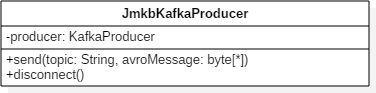
\includegraphics[width=0.5\linewidth]{images/bridge/classes/JmkbKafkaProducer}
\end{figure}
\subsubsection{Declaration}{
\begin{lstlisting}[frame=none]
public class JmkbKafkaProducer
 extends java.lang.Object\end{lstlisting}
\subsubsection{Constructor summary}{
\begin{verse}
\hyperlink{Bridge.JmkbKafkaProducer()}{{\bf JmkbKafkaProducer()}} Default constructor\\
\end{verse}
}
\subsubsection{Method summary}{
\begin{verse}
\hyperlink{Bridge.JmkbKafkaProducer.disconnect()}{{\bf disconnect()}} Disconnects this Kafka producer from the Kafka Cluster and closes the producer.\\
\hyperlink{Bridge.JmkbKafkaProducer.send(java.lang.String, byte[])}{{\bf send(String, byte\lbrack \rbrack )}} Asynchronously sends a record to the topic.\\
\end{verse}
}
\subsubsection{Constructors}{
\vskip -2em
\begin{itemize}
\item{ 
\index{JmkbKafkaProducer()}
\hypertarget{Bridge.JmkbKafkaProducer()}{{\bf  JmkbKafkaProducer}\\}
\begin{lstlisting}[frame=none]
public JmkbKafkaProducer()\end{lstlisting} %end signature
\begin{itemize}
\item{
{\bf  Description}

Default constructor
}
\end{itemize}
}%end item
\end{itemize}
}
\subsubsection{Methods}{
\vskip -2em
\begin{itemize}
\item{ 
\index{disconnect()}
\hypertarget{Bridge.JmkbKafkaProducer.disconnect()}{{\bf  disconnect}\\}
\begin{lstlisting}[frame=none]
public void disconnect()\end{lstlisting} %end signature
\begin{itemize}
\item{
{\bf  Description}

Disconnects this Kafka producer from the Kafka Cluster and closes the producer.
}
\end{itemize}
}%end item
\item{ 
\index{send(String, byte\lbrack \rbrack )}
\hypertarget{Bridge.JmkbKafkaProducer.send(java.lang.String, byte[])}{{\bf  send}\\}
\begin{lstlisting}[frame=none]
public void send(java.lang.String topic,byte[] avroMessage)\end{lstlisting} %end signature
\begin{itemize}
\item{
{\bf  Description}

Asynchronously sends a record to the topic.
}
\item{
{\bf  Parameters}
  \begin{itemize}
   \item{
\texttt{topic} -- The topic.}
   \item{
\texttt{avroMessage} -- The message to send.}
  \end{itemize}
}%end item
\end{itemize}
}%end item
\end{itemize}
}
}
\subsection{\label{Bridge.JmkbMqttConsumer}Class JmkbMqttConsumer}{
\hypertarget{Bridge.JmkbMqttConsumer}{}\vskip .1in 
This class serves as an MqttClient that consumes messages from the specified FROST-Server address. On message arrival, it will initiate the conversion of the message to a desired format via MqttMessageConverter and supply the converted message to a JmkbKafkaProducer. An instance of this class should be destroyed with a call to the disconnect() method.\vskip .1in 
\subsubsection{Declaration}{
\begin{lstlisting}[frame=none]
public class JmkbMqttConsumer
 extends java.lang.Object\end{lstlisting}
\subsubsection{Constructor summary}{
\begin{verse}
\hyperlink{Bridge.JmkbMqttConsumer()}{{\bf JmkbMqttConsumer()}} Default constructor\\
\end{verse}
}
\subsubsection{Method summary}{
\begin{verse}
\hyperlink{Bridge.JmkbMqttConsumer.connectionLost(java.lang.Throwable)}{{\bf connectionLost(Throwable)}} This method is called when the connection to the server is lost.\\
\hyperlink{Bridge.JmkbMqttConsumer.deliveryComplete(IMqttDeliveryToken)}{{\bf deliveryComplete(IMqttDeliveryToken)}} Called when delivery for a message has been completed, and all acknowledgments have been received.\\
\hyperlink{Bridge.JmkbMqttConsumer.disconnect()}{{\bf disconnect()}} Disconnects client from MQTT and closes the client.\\
\hyperlink{Bridge.JmkbMqttConsumer.JmkbMqttConsumer(java.lang.String, Bridge.JmkbKafkaProducer)}{{\bf JmkbMqttConsumer(String, JmkbKafkaProducer)}} This constructor for this class.\\
\hyperlink{Bridge.JmkbMqttConsumer.messageArrived(java.lang.String, MqttMessage)}{{\bf messageArrived(String, MqttMessage)}} This method is called when a message arrives from the server.\\
\end{verse}
}
\subsubsection{Constructors}{
\vskip -2em
\begin{itemize}
\item{ 
\index{JmkbMqttConsumer()}
\hypertarget{Bridge.JmkbMqttConsumer()}{{\bf  JmkbMqttConsumer}\\}
\begin{lstlisting}[frame=none]
public JmkbMqttConsumer()\end{lstlisting} %end signature
\begin{itemize}
\item{
{\bf  Description}

Default constructor
}
\end{itemize}
}%end item
\end{itemize}
}
\subsubsection{Methods}{
\vskip -2em
\begin{itemize}
\item{ 
\index{connectionLost(Throwable)}
\hypertarget{Bridge.JmkbMqttConsumer.connectionLost(java.lang.Throwable)}{{\bf  connectionLost}\\}
\begin{lstlisting}[frame=none]
public void connectionLost(java.lang.Throwable cause)\end{lstlisting} %end signature
\begin{itemize}
\item{
{\bf  Description}

This method is called when the connection to the server is lost.
}
\item{
{\bf  Parameters}
  \begin{itemize}
   \item{
\texttt{cause} -- the reason behind the loss of connection.}
  \end{itemize}
}%end item
\end{itemize}
}%end item
\item{ 
\index{deliveryComplete(IMqttDeliveryToken)}
\hypertarget{Bridge.JmkbMqttConsumer.deliveryComplete(IMqttDeliveryToken)}{{\bf  deliveryComplete}\\}
\begin{lstlisting}[frame=none]
public void deliveryComplete(IMqttDeliveryToken token)\end{lstlisting} %end signature
\begin{itemize}
\item{
{\bf  Description}

Called when delivery for a message has been completed, and all acknowledgments have been received. In this implementation of this method, nothing happens.
}
\item{
{\bf  Parameters}
  \begin{itemize}
   \item{
\texttt{token} -- the delivery token associated with the message.}
  \end{itemize}
}%end item
\end{itemize}
}%end item
\item{ 
\index{disconnect()}
\hypertarget{Bridge.JmkbMqttConsumer.disconnect()}{{\bf  disconnect}\\}
\begin{lstlisting}[frame=none]
public void disconnect()\end{lstlisting} %end signature
\begin{itemize}
\item{
{\bf  Description}

Disconnects client from MQTT and closes the client.
}
\end{itemize}
}%end item
\item{ 
\index{JmkbMqttConsumer(String, JmkbKafkaProducer)}
\hypertarget{Bridge.JmkbMqttConsumer.JmkbMqttConsumer(java.lang.String, Bridge.JmkbKafkaProducer)}{{\bf  JmkbMqttConsumer}\\}
\begin{lstlisting}[frame=none]
public void JmkbMqttConsumer(java.lang.String clientId,JmkbKafkaProducer producer)\end{lstlisting} %end signature
\begin{itemize}
\item{
{\bf  Description}

This constructor for this class. Creates a new MqttClient and subscribes to the topics specified in the SensorThings API standard. A unique identifier and a JmkbKafkaProducer should be supplied.
}
\item{
{\bf  Parameters}
  \begin{itemize}
   \item{
\texttt{clientId} -- The unique identifier for the MqttClient.}
   \item{
\texttt{producer} -- A JmkbKafkaProducer.}
  \end{itemize}
}%end item
\end{itemize}
}%end item
\item{ 
\index{messageArrived(String, MqttMessage)}
\hypertarget{Bridge.JmkbMqttConsumer.messageArrived(java.lang.String, MqttMessage)}{{\bf  messageArrived}\\}
\begin{lstlisting}[frame=none]
public void messageArrived(java.lang.String topic,MqttMessage message)\end{lstlisting} %end signature
\begin{itemize}
\item{
{\bf  Description}

This method is called when a message arrives from the server. This method is invoked synchronously by the MQTT client. An acknowledgment is not sent back to the server until this method returns cleanly. Any additional messages which arrive while this method is running will build up in memory, and will then back up on the network. When this method is called, the supplied message will be converted to an Avro message and forwarded to an instance of JmkbKafkaProducer, which will then send the message to the Kafka Cluster.
}
\item{
{\bf  Parameters}
  \begin{itemize}
   \item{
\texttt{topic} -- name of the topic on the message was published to}
   \item{
\texttt{message} -- the actual message.}
  \end{itemize}
}%end item
\end{itemize}
}%end item
\end{itemize}
}
}
\subsection{\label{Bridge.MessageConverter}Class MessageConverter}{
\hypertarget{Bridge.MessageConverter}{}\vskip .1in 
This convenience class provides static methods to convert a given message to another format.\vskip .1in 
\subsubsection{Declaration}{
\begin{lstlisting}[frame=none]
public class MessageConverter
 extends java.lang.Object\end{lstlisting}
\subsubsection{Constructor summary}{
\begin{verse}
\hyperlink{Bridge.MessageConverter()}{{\bf MessageConverter()}} Default constructor\\
\end{verse}
}
\subsubsection{Method summary}{
\begin{verse}
\hyperlink{Bridge.MessageConverter.getSensorIdFromMessage(byte[])}{{\bf getSensorIdFromMessage(byte\lbrack \rbrack )}} This method returns the sensor ID that has supplied the information in the message.\\
\hyperlink{Bridge.MessageConverter.mqttMessageToAvro(MqttMessage)}{{\bf mqttMessageToAvro(MqttMessage)}} This method converts a given MqttMessage, which contains information in the JSON format, to an Avro message in a byte array.\\
\end{verse}
}
\subsubsection{Constructors}{
\vskip -2em
\begin{itemize}
\item{ 
\index{MessageConverter()}
\hypertarget{Bridge.MessageConverter()}{{\bf  MessageConverter}\\}
\begin{lstlisting}[frame=none]
public MessageConverter()\end{lstlisting} %end signature
\begin{itemize}
\item{
{\bf  Description}

Default constructor
}
\end{itemize}
}%end item
\end{itemize}
}
\subsubsection{Methods}{
\vskip -2em
\begin{itemize}
\item{ 
\index{getSensorIdFromMessage(byte\lbrack \rbrack )}
\hypertarget{Bridge.MessageConverter.getSensorIdFromMessage(byte[])}{{\bf  getSensorIdFromMessage}\\}
\begin{lstlisting}[frame=none]
public static java.lang.String getSensorIdFromMessage(byte[] message)\end{lstlisting} %end signature
\begin{itemize}
\item{
{\bf  Description}

This method returns the sensor ID that has supplied the information in the message. In detail, this method searches for the key 'iot.id' in the message and returns the value associated with the key.
}
\item{
{\bf  Parameters}
  \begin{itemize}
   \item{
\texttt{message} -- The message from which to extract the sensor ID.}
  \end{itemize}
}%end item
\item{{\bf  Returns} -- 
The sensor ID. 
}%end item
\end{itemize}
}%end item
\item{ 
\index{mqttMessageToAvro(MqttMessage)}
\hypertarget{Bridge.MessageConverter.mqttMessageToAvro(MqttMessage)}{{\bf  mqttMessageToAvro}\\}
\begin{lstlisting}[frame=none]
public static byte[] mqttMessageToAvro(MqttMessage message)\end{lstlisting} %end signature
\begin{itemize}
\item{
{\bf  Description}

This method converts a given MqttMessage, which contains information in the JSON format, to an Avro message in a byte array.
}
\item{
{\bf  Parameters}
  \begin{itemize}
   \item{
\texttt{message} -- The message to convert.}
  \end{itemize}
}%end item
\item{{\bf  Returns} -- 
The message in Avro format. 
}%end item
\end{itemize}
}%end item
\end{itemize}
}
}
\subsection{\label{Bridge.PropertiesFileReader}Class PropertiesFileReader}{
\hypertarget{Bridge.PropertiesFileReader}{}\vskip .1in 
A class that reads properties from the configuration file (jmkb.properties) and provides a method for getting a property by key.\vskip .1in 
\subsubsection{Declaration}{
\begin{lstlisting}[frame=none]
public class PropertiesFileReader
 extends java.lang.Object\end{lstlisting}
\subsubsection{Constructor summary}{
\begin{verse}
\hyperlink{Bridge.PropertiesFileReader()}{{\bf PropertiesFileReader()}} Default constructor\\
\end{verse}
}
\subsubsection{Method summary}{
\begin{verse}
\hyperlink{Bridge.PropertiesFileReader.getProperty(java.lang.String)}{{\bf getProperty(String)}} Searches for the property with the specified key in jmkb.property.\\
\end{verse}
}
\subsubsection{Constructors}{
\vskip -2em
\begin{itemize}
\item{ 
\index{PropertiesFileReader()}
\hypertarget{Bridge.PropertiesFileReader()}{{\bf  PropertiesFileReader}\\}
\begin{lstlisting}[frame=none]
public PropertiesFileReader()\end{lstlisting} %end signature
\begin{itemize}
\item{
{\bf  Description}

Default constructor
}
\end{itemize}
}%end item
\end{itemize}
}
\subsubsection{Methods}{
\vskip -2em
\begin{itemize}
\item{ 
\index{getProperty(String)}
\hypertarget{Bridge.PropertiesFileReader.getProperty(java.lang.String)}{{\bf  getProperty}\\}
\begin{lstlisting}[frame=none]
public void getProperty(java.lang.String key)\end{lstlisting} %end signature
\begin{itemize}
\item{
{\bf  Description}

Searches for the property with the specified key in jmkb.property.
}
\item{
{\bf  Parameters}
  \begin{itemize}
   \item{
\texttt{key} -- The value associated with the key or null if the key is not found.}
  \end{itemize}
}%end item
\end{itemize}
}%end item
\end{itemize}
}
}
\subsection{\label{Bridge.SchemaRegistryConnector}Class SchemaRegistryConnector}{
\hypertarget{Bridge.SchemaRegistryConnector}{}\vskip .1in 
Convenience class which provides methods for interacting with the schema registry.\vskip .1in 
\subsubsection{Declaration}{
\begin{lstlisting}[frame=none]
public class SchemaRegistryConnector
 extends java.lang.Object\end{lstlisting}
\subsubsection{Constructor summary}{
\begin{verse}
\hyperlink{Bridge.SchemaRegistryConnector()}{{\bf SchemaRegistryConnector()}} Default constructor\\
\end{verse}
}
\subsubsection{Method summary}{
\begin{verse}
\hyperlink{Bridge.SchemaRegistryConnector.getSchemaById(int)}{{\bf getSchemaById(int)}} Requests the schema associated with the schema ID from the schema registry.\\
\hyperlink{Bridge.SchemaRegistryConnector.getSchemaBySubject(java.lang.String)}{{\bf getSchemaBySubject(String)}} Requests the latest version of the schema associated with the given subject from the schema registry.\\
\hyperlink{Bridge.SchemaRegistryConnector.getSchemaBySubject(java.lang.String, int)}{{\bf getSchemaBySubject(String, int)}} Requests the given version of the schema associated with the given subject from the schema registry.\\
\end{verse}
}
\subsubsection{Constructors}{
\vskip -2em
\begin{itemize}
\item{ 
\index{SchemaRegistryConnector()}
\hypertarget{Bridge.SchemaRegistryConnector()}{{\bf  SchemaRegistryConnector}\\}
\begin{lstlisting}[frame=none]
public SchemaRegistryConnector()\end{lstlisting} %end signature
\begin{itemize}
\item{
{\bf  Description}

Default constructor
}
\end{itemize}
}%end item
\end{itemize}
}
\subsubsection{Methods}{
\vskip -2em
\begin{itemize}
\item{ 
\index{getSchemaById(int)}
\hypertarget{Bridge.SchemaRegistryConnector.getSchemaById(int)}{{\bf  getSchemaById}\\}
\begin{lstlisting}[frame=none]
public java.lang.String getSchemaById(int id)\end{lstlisting} %end signature
\begin{itemize}
\item{
{\bf  Description}

Requests the schema associated with the schema ID from the schema registry. Returns the schema if successful, null if not.
}
\item{
{\bf  Parameters}
  \begin{itemize}
   \item{
\texttt{id} -- The schema id.}
  \end{itemize}
}%end item
\item{{\bf  Returns} -- 
The schema if successful, null if not. 
}%end item
\end{itemize}
}%end item
\item{ 
\index{getSchemaBySubject(String)}
\hypertarget{Bridge.SchemaRegistryConnector.getSchemaBySubject(java.lang.String)}{{\bf  getSchemaBySubject}\\}
\begin{lstlisting}[frame=none]
public java.lang.String getSchemaBySubject(java.lang.String subject)\end{lstlisting} %end signature
\begin{itemize}
\item{
{\bf  Description}

Requests the latest version of the schema associated with the given subject from the schema registry. Returns the schema if successful, null if not.
}
\item{
{\bf  Parameters}
  \begin{itemize}
   \item{
\texttt{subject} -- The subject of the schema.}
  \end{itemize}
}%end item
\item{{\bf  Returns} -- 
The schema if successful, null if not. 
}%end item
\end{itemize}
}%end item
\item{ 
\index{getSchemaBySubject(String, int)}
\hypertarget{Bridge.SchemaRegistryConnector.getSchemaBySubject(java.lang.String, int)}{{\bf  getSchemaBySubject}\\}
\begin{lstlisting}[frame=none]
public java.lang.String getSchemaBySubject(java.lang.String subject,int version)\end{lstlisting} %end signature
\begin{itemize}
\item{
{\bf  Description}

Requests the given version of the schema associated with the given subject from the schema registry. Returns the schema if successful, null if not.
}
\item{
{\bf  Parameters}
  \begin{itemize}
   \item{
\texttt{subject} -- The subject of the schema.}
   \item{
\texttt{version} -- The schema version.}
  \end{itemize}
}%end item
\item{{\bf  Returns} -- 
the schema if successful, null if not. 
}%end item
\end{itemize}
}%end item
\end{itemize}
}
}
}
